\documentclass[a4paper,indent]{paper}
\usepackage{tikz}
\usepackage{microtype}
\usepackage{inputenc}
\usepackage{rotating}
\usepackage{fullpage}
\usepackage{caption}
\usepackage{tikz}
\usepackage{tikz-timing}
\usepackage{mdframed}
\usepackage{fourier} % for /danger
\usepackage{amsmath}
\usepackage{acronym}
\usepackage[hidelinks]{hyperref}

\usetikzlibrary{arrows, shapes.gates.logic.US, calc}
%\usetikzlibrary{external} % doesn't work with tikz timing diagrams
%\tikzexternalize % activate!

\title{Auger Radio Digitizer}
\subtitle{Software Developer's Guide}
\author{%
  Sjoerd T. Timmer (s.timmer@astro.ru.nl)}
\date{}


\acrodef{RD}[RD]{Radio Digitizer}
\acrodef{UUB}[UUB]{Universal Upgrade Board}
\acrodef{SPI}[SPI]{Serial Peripheral Interface}
\acrodef{ADC}[ADC]{analog-to-digital converter}
\acrodef{FPGA}[FPGA]{field programmable gate array}
\acrodef{DDR}[DDR]{double data rate}
\acrodef{GPIO}[GPIO]{general-purpose IO}
\acrodef{LNA}[LNA]{low-noise amplifier}
\acrodef{PGA}[PGA]{programmable-gain amplifier}
\acrodef{MSB}[MSB]{most-significant bit}
\acrodef{I2C}[$\text{I}^2\text{C}$]{}
\acused{I2C}
%\newmdenv[linecolor=orange,backgroundcolor=orange!10]{warning}

\newenvironment{warning}
{\par\begin{mdframed}[linewidth=2pt,linecolor=orange,backgroundcolor=orange!10]%
    \begin{list}{}{\leftmargin=0mm}\item[\bf\danger{}~~Warning: ]}
  {\end{list}\end{mdframed}\par}

\begin{document}
\maketitle{}
\begin{abstract}
  This document describes the internal firmware architecture of the Auger \acf{RD} module. \acresetall
\end{abstract}

\begin{mdframed}[linewidth=2pt,linecolor=orange,backgroundcolor=orange!10]%
  This document is work-in-progress.
  It described both the currently implemented state of affairs as well as the intended final implementation.
  At the time of this writing (December 2019) some details, in particular relating to the housekeeping interface, are not yet finalized and are subject to change. Note the warning boxes in the relevant sections. 
\end{mdframed}
  
\tableofcontents

\clearpage


\section{Developers Guide/Architecture}
\subsection{General architecture}
\subsubsection{\acs{SPI} demux}

\subsubsection{Boot sequence injection}


\subsection{Housekeeping sub-systems}

\subsubsection{Program flash (0x02)}

\subsubsection{Science \acs{ADC} (0x03)}

\subsubsection{Current and voltage monitoring (0x04)}

\subsubsection{Temperature sensor (0x05)}

\subsubsection{Trigger injection (0x06)}

\subsubsection{Firmware version register (0x07)}

\subsubsection{Trigger-offset register (0x08)}

\subsubsection{Raw data capture (0x12)}

\begin{warning}
  This sub-system is not compiled in the default distributed firmware. It can be enabled in housekeeping.vhd.
\end{warning}

Raw data capture allows reading of the ADC data via the housekeeping interface.
This is completely separate from the science acquisition process.
It neither relies on, nor interferes with the normal trigger and transfer processes.
The data is stored in a separate buffer.

Upto 8192 samples can be retrieved. If the \ac{SPI} transaction continues after that the first samples will be re-transmitted. Note that due to the nature of the \spi{ADC} data alignment the order of the samples is:
$$
\ldots \text{channel A sample } n \Rightarrow \text{channel B sample } n \Rightarrow \text{channel A sample } n+1 \Rightarrow \text{channel B sample } n+1 => \ldots
$$

Each sample contains 13 bits. The first bit is the value of a digital pin on the \ac{FPGA} which can be used to calibrate the phase of the received signal. Note that these bits in channel B are sampled at the falling clock edges of the 250MHz sample clock and that the digital pin is effectively sampled at 500MHz. The last 12 bits are the sample value. Like the science data it is transferred MSB-first and in 2's-complement. 

It is safe to abort the \ac{SPI} transfer before the end of the buffer. The capture will restart to run as soon as CE is released. Note that there is no mechanisms to prevent overlapping transfers from producing corrupted traces. I.e., to be sure to capture a clean trace, wait at least $8192/250 (MHz) \simeq 33 (us)$ after the release of the CE before pulling it low again (including the subsystem selection byte).

\subsection{\acs{ADC} driver}
The adc\_driver converts the 12 \ac{DDR} 250 MHz data lines to 48 `normal' data lines at 125MHz.
At each clock cycle 2 samples are produced for each of the 2 channels.
In the ADS4229 datasheet we find that the bits of the samples are organized slightly differently than the output of the auto-generated adc\_driver block produces them:

\begin{center}
  \begin{tabular}{l|l|l}
    RD & ADC & timing\\\hline
    \multicolumn{2}{l|}{250 MHz clk}  & \texttiming[timing/wscale=9]{LHLHL0.04H}\\
    \multicolumn{2}{l|}{125 MHz clk} & \texttiming[timing/wscale=9]{L2H2L0.04H}\vspace*{2mm}\\
    D0  & DA0   & \texttiming[timing/wscale=9]{u[fill=green!30]D{Q[0]=S[A][2k][0]}[fill=green!30]D{Q[13]=S[A][2k][1]}[fill=orange!30]D{Q[26]=S[A][2k+1][0]}[fill=orange!30]D{Q[39]=S[A][2k+1][1]}[fill=gray]u}\\
    D1  & DA2   & \texttiming[timing/wscale=9]{u[fill=green!30]D{Q[1]=S[A][2k][2]}[fill=green!30]D{Q[14]=S[A][2k][3]}[fill=orange!30]D{Q[27]=S[A][2k+1][2]}[fill=orange!30]D{Q[40]=S[A][2k+1][3]}[fill=gray]u}\\
    D2  & DA4   & \texttiming[timing/wscale=9]{u[fill=green!30]D{Q[2]=S[A][2k][4]}[fill=green!30]D{Q[15]=S[A][2k][5]}[fill=orange!30]D{Q[28]=S[A][2k+1][4]}[fill=orange!30]D{Q[41]=S[A][2k+1][5]}[fill=gray]u}\\
    D3  & DA6   & \texttiming[timing/wscale=9]{u[fill=green!30]D{Q[3]=S[A][2k][6]}[fill=green!30]D{Q[16]=S[A][2k][7]}[fill=orange!30]D{Q[29]=S[A][2k+1][6]}[fill=orange!30]D{Q[42]=S[A][2k+1][7]}[fill=gray]u}\\
    D4  & DA8   & \texttiming[timing/wscale=9]{u[fill=green!30]D{Q[4]=S[A][2k][8]}[fill=green!30]D{Q[17]=S[A][2k][9]}[fill=orange!30]D{Q[30]=S[A][2k+1][8]}[fill=orange!30]D{Q[43]=S[A][2k+1][9]}[fill=gray]u}\\
    D5  & FA10  & \texttiming[timing/wscale=9]{u[fill=green!30]D{Q[5]=S[A][2k][10]}[fill=green!30]D{Q[18]=S[A][2k][11]}[fill=orange!30]D{Q[31]=S[A][2k+1][10]}[fill=orange!30]D{Q[44]=S[A][2k+1][11]}[fill=gray]u}    \vspace*{2mm}\\
    D6  & DB0   & \texttiming[timing/wscale=9]{u[fill=blue!30]D{Q[6]=S[B][2k][0]}[fill=blue!30]D{Q[19]=S[B][2k][1]}[fill=red!30]D{Q[32]=S[B][2k+1][0]}[fill=red!30]D{Q[45]=S[B][2k+1][1]}[fill=gray]u}\\
    D7  & DB2   & \texttiming[timing/wscale=9]{u[fill=blue!30]D{Q[7]=S[B][2k][2]}[fill=blue!30]D{Q[20]=S[B][2k][3]}[fill=red!30]D{Q[33]=S[B][2k+1][2]}[fill=red!30]D{Q[46]=S[B][2k+1][3]}[fill=gray]u}\\
    D8  & DB4   & \texttiming[timing/wscale=9]{u[fill=blue!30]D{Q[8]=S[B][2k][4]}[fill=blue!30]D{Q[21]=S[B][2k][5]}[fill=red!30]D{Q[34]=S[B][2k+1][4]}[fill=red!30]D{Q[47]=S[B][2k+1][5]}[fill=gray]u}\\
    D9  & DB6   & \texttiming[timing/wscale=9]{u[fill=blue!30]D{Q[9]=S[B][2k][6]}[fill=blue!30]D{Q[22]=S[B][2k][7]}[fill=red!30]D{Q[35]=S[B][2k+1][6]}[fill=red!30]D{Q[48]=S[B][2k+1][7]}[fill=gray]u}\\
    D10 & DB8   & \texttiming[timing/wscale=9]{u[fill=blue!30]D{Q[10]=S[B][2k][8]}[fill=blue!30]D{Q[23]=S[B][2k][9]}[fill=red!30]D{Q[36]=S[B][2k+1][8]}[fill=red!30]D{Q[49]=S[B][2k+1][9]}[fill=gray]u}\\
    D11 & FB10  & \texttiming[timing/wscale=9]{u[fill=blue!30]D{Q[11]=S[B][2k][10]}[fill=blue!30]D{Q[24]=S[B][2k][11]}[fill=red!30]D{Q[37]=S[B][2k+1][10]}[fill=red!30]D{Q[50]=S[B][2k+1][11]}[fill=gray]u}    \vspace*{2mm}\\
    \multicolumn{2}{l|}{trigger}    & \texttiming[timing/wscale=9]{u[fill=green!30]D{Q[12]}[fill=blue!30]D{Q[25]}[fill=orange!30]D{Q[38]}[fill=red!30]D{Q[51]}[fill=gray]u}\\
  \end{tabular}
  \captionof{figure}{Adc\_driver output format. Q is the data format of the adc\_driver output. S is the data format of the ADC. Note that for historical compatibility channel A on the ADC is channel 2 of the RD and channel B on the ADC is channel 1 of the RD. The four samples that are processed by the RD simultaneously have been color coded. The trigger signal is sampled with the ADC data but it is not actually transmitted with the samples.}
\end{center}


Note that the trigger input is used as the 13th input to the \ac{DDR} decoder.
This provides four synchonized samples of the trigger input.
The last sample (q[51]) is used to trigger the write\_controller.
The second (q[25]) is used to determine if the even or odd sample will be used as the first (and last) sample in the trace.
The sub-sample trigger information (q[12] \textbf{xor} q[25] \textbf{xor} q[36]) can be retrieved through the housekeeping \ac{SPI} interface.

\begin{warning}
  The retrieval of the sub-sample trigger information is not actually implemented at the time of this writing.
\end{warning}





\subsubsection{Write Controller}
%The write controller is responsible for enabling and disabling writes to the circular buffer.
%It listens in on the address counter ($i\_curr\_address$) and controls (besides the write enable ($o\_write\_enable$)) the start ($o\_trigger\_done$) and trigger-offset ($o\_start\_addr$) of the Readout Controller.
%
%A configurable trigger-offset ($i\_start\_offset$) determines how many samples are stored before the trigger.
%In the current instantiation the address width is eleven bits so there are 2048 samples and therefore $2048 - i\_start\_offset$ samples after the trigger.
%
%
%The Write Controller needs to be enabled with a pulse on the $i\_arm$ input.
%After this pulse the Write Controller will enable writes within 2 clock cycles.
%
%The \ac{ADC} driver outputs 2 samples in each clock cycle (for each channel, so 4 in total at each clock cycle).
%Therefore the Write Controller should wait for at least
%$$
%\left\lceil\frac{i\_start\_offset}{2}\right\rceil
%$$
%clock cycles  before accepting triggers.
%
%After the trigger is first seen high, the Write Controller should keep $o\_write\_enable$ high for exactly
%$$
%\left\lceil\frac{2048 - i\_start\_offset}{2}\right\rceil
%$$
%clock cycles. At that time $o\_write\_enable$ has to be asserted low and $o\_trigger\_done$ should be asserted high. At that time $o\_start\_addr$ has to be set to the address at which the data starts:
%$$
%i\_curr\_addr - i\_start\_offset \pmod{2048}
%$$
%This condition should hold until the next pulse on the $i\_arm$ signal.
%
%
%A trigger-offset of 0 (or 1) is considered invalid but anything in the closed interval $[1, 2047]$ should work.
%



\subsubsection{Trigger injection through housekeeping \ac{SPI}}
\begin{warning}
  This \ac{SPI} sub-system is candidate for removal in the next release.
  This address 0x06 may become a trigger for the \ac{I2C} readout instead.
\end{warning}

There is an \ac{SPI} sub-system at address 0x06 that can be used to trigger the \ac{RD} if no external trigger is present.
This is useful for debugging.
The inverted CE of this submodule is or'ed with the external trigger input. It is not necessary to send any data for the trigger to work.
\begin{center}
  \begin{tikztimingtable}[timing/wscale=1]
    clk    & HHCCCCCCCCCCCCCCCCHH \\
    ce     & HHLLLLLLLLLLLLLLLLHH \\
    mosi   & UUDDDDDDDDDDDDDDDD{0x06 (internal trigger)}UU \\
    trig\_int & HHHHHHHHHHHHHHHHHLHH \\
  \end{tikztimingtable}
  \captionof{figure}{Example transaction to inject an internal trigger.}
\end{center}
\begin{center}
  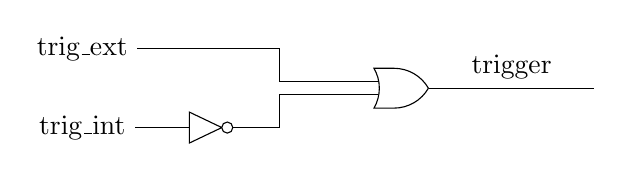
\begin{tikzpicture}
    \node (te) at (0, 1) {trig\_ext};
    \node (ti) at (0, 0) {trig\_int};
    \node[not gate US, draw] at ($(ti) + (1.5, 0)$) (notti) {};
    \node[or gate US, draw, rotate=0, logic gate inputs=nn] at ($(notti) + (2.5, 0.5)$) (teornotti) {};
    \draw (ti) -- (notti.input);
    \draw (te) -- (2.5,1) |- (teornotti.input 1);
    \draw (notti.output) -- (2.5,0) |- (teornotti.input 2);
    \draw (teornotti.output) -- node[above]{trigger} ($(teornotti) + (2.5, 0)$);
  \end{tikzpicture}
  \captionof{figure}{Internal wiring of internal and external trigger.}
\end{center}





\end{document}